Dans cette section, nous présentons les principales interfaces réalisées au cours du sprint 1.2. 
\begin{itemize}[label=$\bullet$]
    \item \textbf{Interface de configuration des paramètres de scan}:
    La figure \ref{fig:interface_parametres_scan}\footnote{Voir Annexe E, figure \ref{fig:interface_parametres_scan}} illustre l’interface permettant de personnaliser les paramètres d’un scan. Celle-ci permet à l’utilisateur de définir la profondeur de l’analyse, d’activer ou non certains modules (comme le spider ou le scan AJAX), ou encore de choisir des options spécifiques à certains outils.
    
    \item \textbf{Interface de sélection des outils de sécurité}:
    La figure \ref{fig:interface_selection_outils} présente l’écran dédié à la sélection des outils de sécurité. Cette interface propose une liste de cases à cocher pour activer ou désactiver les outils disponibles, accompagnée de boutons «Tout sélectionner» et «Tout désélectionner». Les préférences de l’utilisateur sont sauvegardées pour les réutiliser dans les futurs scans.
     \begin{figure}[H]
        \centering
        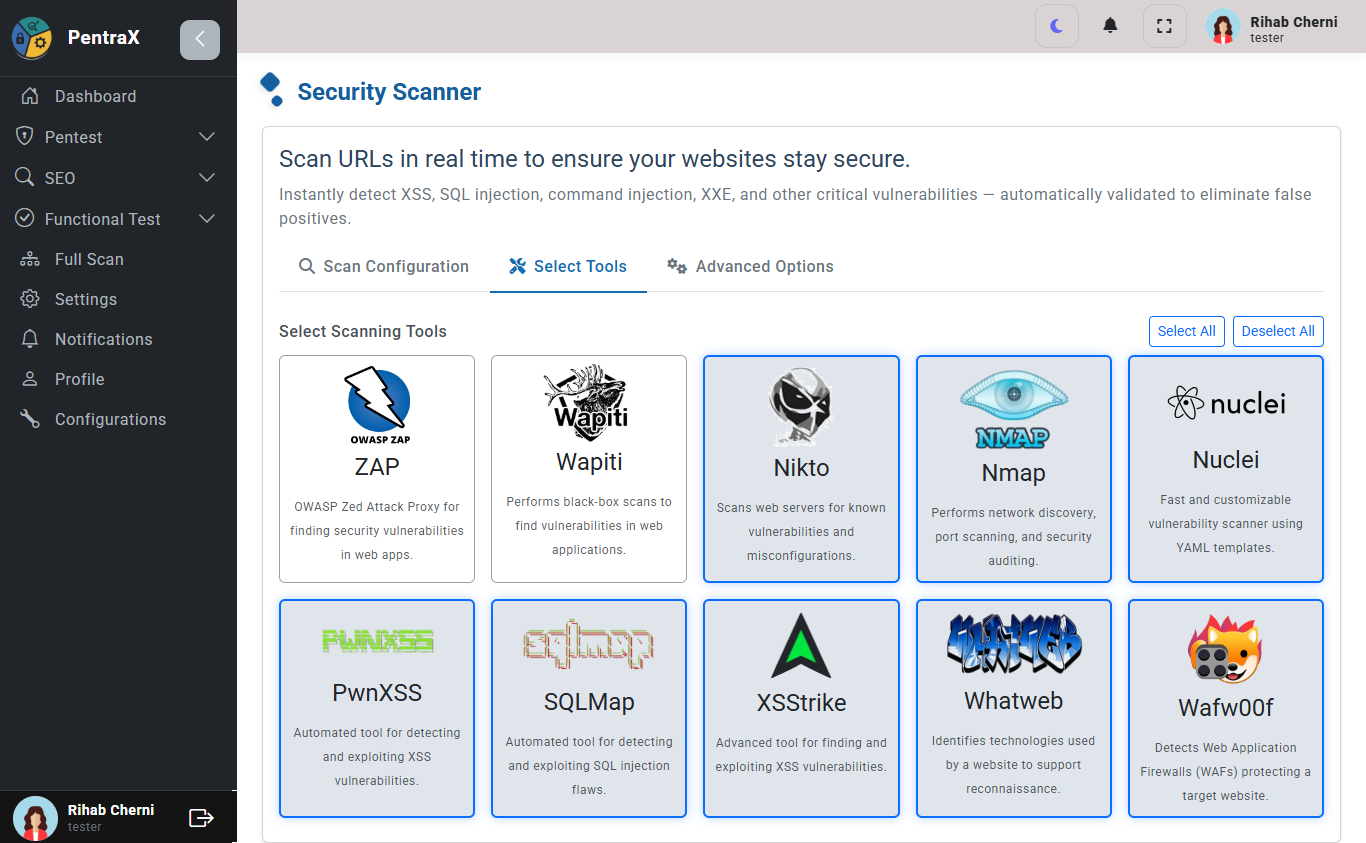
\includegraphics[width=\textwidth]{chapitres/ch3Sp1/section/sprint2/img/interface/tools.png}
        \caption{Interface de sélection des outils de sécurité}
        \label{fig:interface_selection_outils}
    \end{figure}
    \vspace{-0.2cm}
    \item \textbf{Interface utilisateur pour le lancement de scans, avec ou sans authentification} :\\
        La figure \ref{fig:interface_lancement_scan} illustre le formulaire principal de lancement d’un test de sécurité. L’utilisateur y renseigne l’URL de la cible, choisit les outils à utiliser, configure les paramètres du scan, puis lance l’analyse via un bouton dédié.

        Cette interface propose également une section dédiée à l’authentification, activable via des boutons radio. En fonction du type sélectionné, les champs correspondants s’affichent dynamiquement : identifiants (nom d’utilisateur et mot de passe), jetons d’accès (tokens), ou cookies de session. Cette fonctionnalité est essentielle pour analyser les zones protégées d’une application web. Pour plus de détails sur le lancement des scans de sécurité, la gestion des paramètres d’authentification et la configuration des outils, voir l’annexe C\footnote{Voir Annexe C: Automatisation des outils de pentesting}.
        \begin{figure}[H]
            \centering
            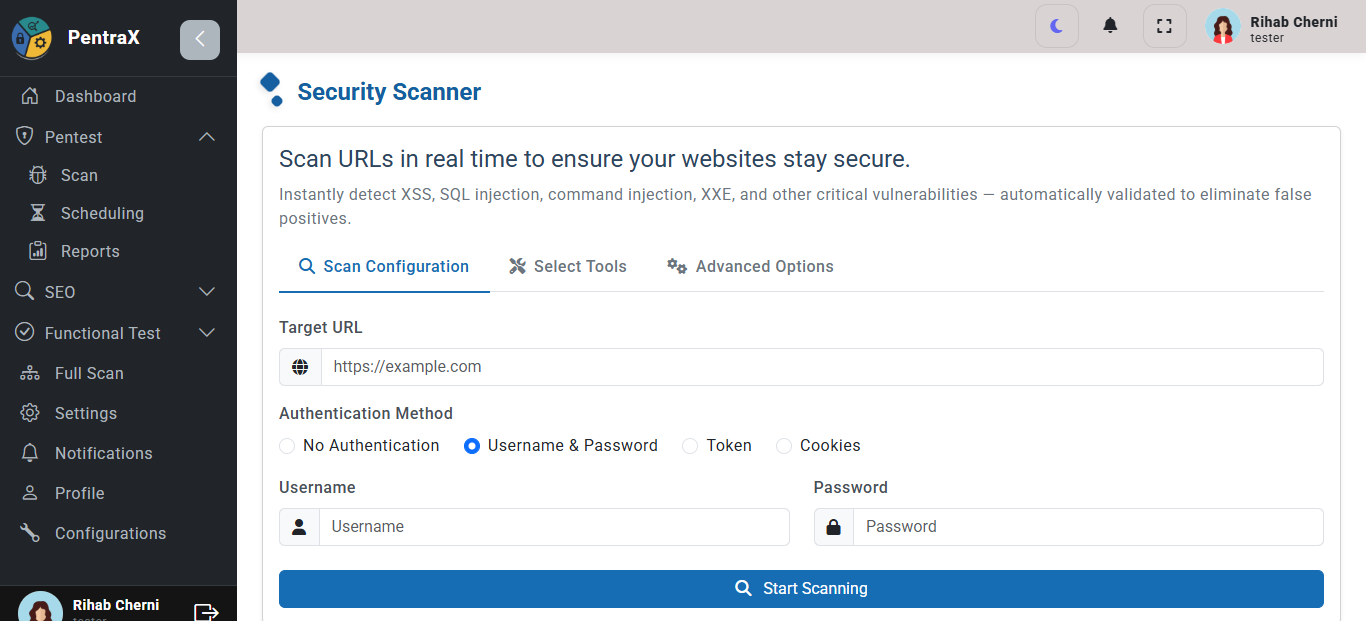
\includegraphics[width=\textwidth]{chapitres/ch3Sp1/section/sprint2/img/interface/start-sca.PNG}
            \caption{Interface de lancement de scan avec ou sans authentification}
            \label{fig:interface_lancement_scan}
        \end{figure}
        \vspace{-0.2cm}
    \item \textbf{Interface de suivi en temps réel des scans}: Comme illustré dans la figure \ref{fig:interface_suivi_ws}\footnote{Voir Annexe E, figure \ref{fig:interface_suivi_ws}}, cette interface permet de suivre l’évolution du scan en temps réel grâce à l’intégration des WebSockets, avec un indicateur de progression affiché de 0 à 100\,\%.    
    \item \textbf{Interface de visualisation des résultats}:
    La figure \ref{fig:interface_resultats_scan} montre l’écran de consultation des vulnérabilités détectées. Des filtres par type, gravité ou outil sont proposés pour affiner l’analyse, et chaque vulnérabilité est accompagnée d’un résumé, de son risque, de sa source et d’une suggestion de correction.
        \begin{figure}[H]
            \centering
            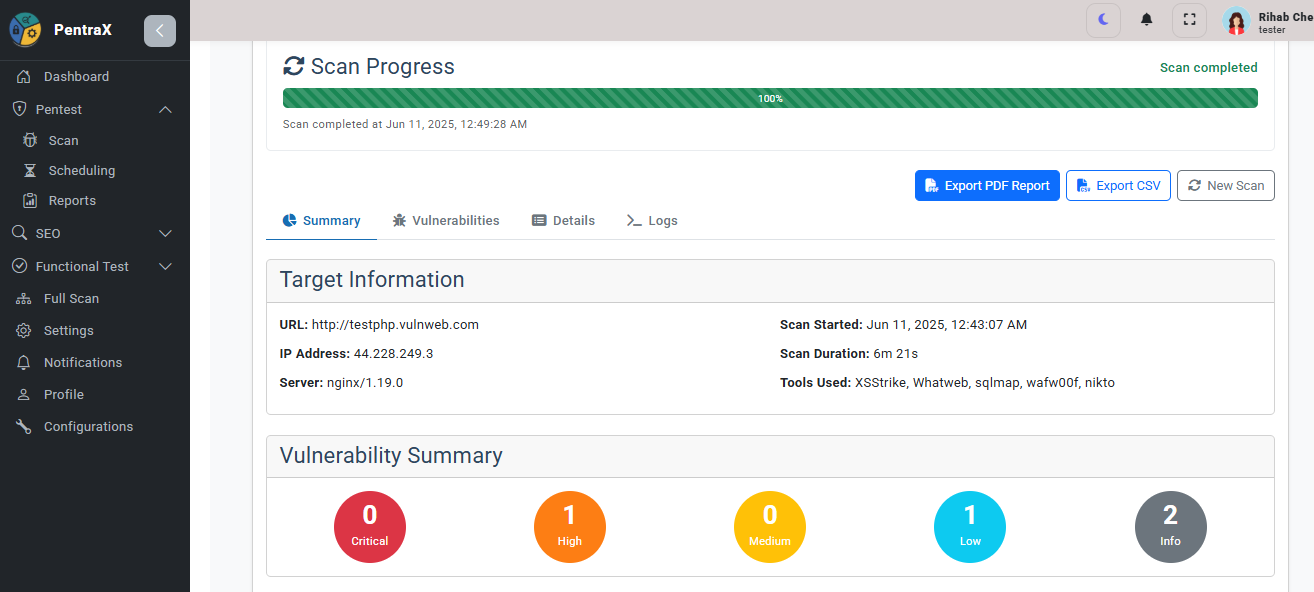
\includegraphics[width=\textwidth]{chapitres/ch3Sp1/section/sprint2/img/interface/res1.PNG}
            \caption{\centering Interface de visualisation des résultats de scan (premier onglet : statistiques et détails techniques)}
            \label{fig:interface_resultats_scan}
        \end{figure}
        \vspace{-0.2cm}
    \item \textbf{Interface de l’historique des scans}:
    L’interface illustrée par la figure \ref{fig:interface_historique_scans}\footnote{Voir Annexe E, figure \ref{fig:interface_historique_scans}} permet d’accéder aux rapports précédemment générés. Une table paginée présente les scans enregistrés, accompagnée de filtres, d’un champ de recherche, et d’une option de suppression.
    
    \item \textbf{Interface de téléchargement des rapports}:
    Comme présenté dans la figure \ref{fig:interface_export_rapports}\footnote{Voir Annexe E, figure \ref{fig:interface_export_rapports}}, cette interface permet de télécharger les rapports aux formats JSON, PDF ou CSV, selon les besoins de l’utilisateur.


    \item \textbf{Interface pour le paramétrage des canaux de diffusion} : La figure \ref{fig:interface_parametrage_canaux}\footnote{Voir Annexe E, figure \ref{fig:interface_parametrage_canaux}} illustre l’interface dédiée à la configuration détaillée des canaux de diffusion des rapports. Elle permet à l’utilisateur de spécifier, pour chaque type de test (sécurité, SEO, fonctionnel), les canaux de notification souhaités (Slack, Jira, Email), le format du rapport associé (PDF, HTML, JSON). Des champs dynamiques permettent d’ajouter plusieurs destinataires e-mail et d’entrer des clés API sécurisées pour Slack et Jira. Cette interface vise à centraliser et automatiser la diffusion ciblée des rapports vers les bons interlocuteurs.

    \item \textbf{Interface d’intégration Jira}:
    La figure \ref{fig:interface_jira_integration}\footnote{Voir Annexe E, figure \ref{fig:interface_jira_integration}} illustre la fonctionnalité d’envoi des vulnérabilités détectées directement vers Jira pour créer automatiquement des tickets. Un aperçu des tickets créés est également affiché.
    
    \item \textbf{Interface de notification Slack et e-mail}:
    Les figures \ref{fig:interface_slack_notification} et \ref{fig:interface_email_notification}\footnote{Voir Annexe E, figures \ref{fig:interface_slack_notification} et \ref{fig:interface_email_notification}} présentent respectivement l’envoi automatique des rapports via Slack et e-mail. Ces notifications sont déclenchées à la fin du scan, contenant un résumé des vulnérabilités et un lien vers le rapport complet.
    
    \item \textbf{Interface de planification automatique des scans}:  
    La figure \ref{fig:interface_planification_scan}\footnote{Voir Annexe E, figure \ref{fig:interface_planification_scan}} illustre l’écran de planification permettant à l’utilisateur de définir des scans récurrents. Il peut spécifier la fréquence (quotidienne, hebdomadaire, mensuelle), l’heure d’exécution, la cible concernée et les paramètres associés. Une liste des tâches planifiées est également visible et modifiable.
    
    \item \textbf{Interface de gestion centralisée des notifications}: La figure \ref{fig:interface_notifications_config}\footnote{Voir Annexe E, figure \ref{fig:interface_notifications_config}} présente une interface unifiée permettant à l’utilisateur d’activer et de configurer les canaux de diffusion des rapports vers Jira, Slack et l’e-mail. L’interface offre des options pour sélectionner les canaux souhaités, saisir les identifiants API (Slack, Jira ou les adresses e-mail), et choisir les formats (HTML, PDF, JSON) ainsi que les types de rapports à transmettre (sécurité, fonctionnel, SEO).
\end{itemize}

